\newpage
\subsection{Allgemeines Dreieck}

\begin{itemize}
    \item $sin(\alpha) = \frac{hc}{b} \rightarrow hc = sin(\alpha)*b \rightarrow hc$
    \item $sin(\beta) = \frac{hc}{a} \rightarrow hc = sin(\beta)*a \rightarrow hc$
    \item $sin(\alpha)*b = sin(\beta)*a$
    \item $\frac{sin(\alpha)}{a} = \frac{sin(\beta)}{b}$
    \item $A=\frac{b*c}{2} * sin(\alpha)$
    \item $A=\frac{a*c}{2} * sin(\beta)$
    \item $A=\frac{a*b}{2} * sin(\gamma)$
\end{itemize}

\hfill \break
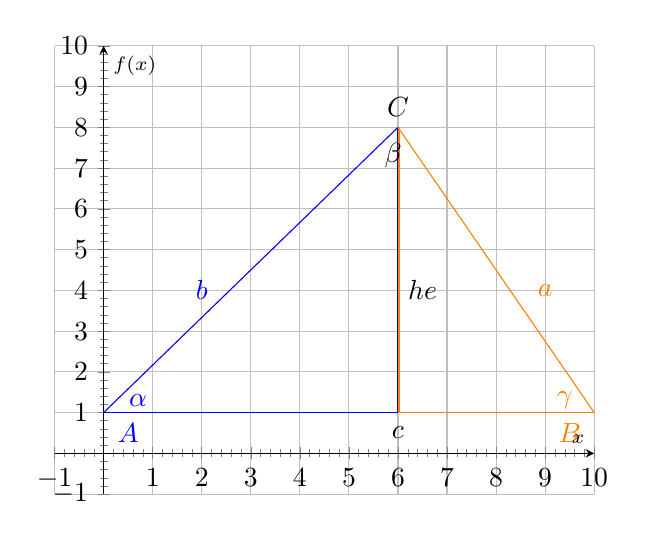
\begin{tikzpicture}[scale=1]
    \begin{axis}%
        [
            grid=major,
            xtick={-1,0,...,10},
            minor x tick num=4,
            xmin=-1,
            xmax=10,
            xlabel={\scriptsize $x$},
            axis x line=middle,
            ytick={-1,0,...,10},
            minor y tick num=4,
            ymin=-1,
            ymax=10,
            ylabel={\scriptsize $f(x)$},
            axis y line=middle,
            no markers,
            samples=100,
            domain=-1:10,
        ]

        \draw[color=blue] (0,1) -- (6,8);
        \draw[color=blue] (0,1) -- (6,1);
        \draw[color=blue] (5.99,1) -- (5.99,8);
        \draw[color=orange] (6.02,1) -- (6.02,8);
        \draw[color=orange] (10,1) -- (6,8);
        \draw[color=orange] (6,1) -- (10,1);

        \node[color=blue] at (0.7,1.3) {$\alpha$};
        \node[color=black] at (5.9,7.3) {$\beta$};
        \node[color=orange] at (9.4,1.3) {$\gamma$};

        \node[color=black] at (6.5,4) {$he$};
        \node[color=orange] at (9,4) {$a$};
        \node[color=blue] at (2,4) {$b$};
        \node[color=black] at (6,0.5) {$c$};

        \node[color=blue] at (0.5,0.5) {$A$};
        \node[color=orange] at (9.5,0.5) {$B$};
        \node[color=black] at (6,8.5) {$C$};
    \end{axis}
\end{tikzpicture}